%
% Libelf by Example
%
% Copyright (c) 2006-2010 Joseph Koshy.  All rights reserved.
%
% Redistribution and use in source and binary forms, with or without
% modification, are permitted provided that the following conditions
% are met:
% 1. Redistributions of source code must retain the above copyright
%    notice, this list of conditions and the following disclaimer.
% 2. Redistributions in binary form must reproduce the above copyright
%    notice, this list of conditions and the following disclaimer in the
%    documentation and/or other materials provided with the distribution.
%
% This software is provided by Joseph Koshy ``as is'' and
% any express or implied warranties, including, but not limited to, the
% implied warranties of merchantability and fitness for a particular purpose
% are disclaimed.  in no event shall Joseph Koshy be liable
% for any direct, indirect, incidental, special, exemplary, or consequential
% damages (including, but not limited to, procurement of substitute goods
% or services; loss of use, data, or profits; or business interruption)
% however caused and on any theory of liability, whether in contract, strict
% liability, or tort (including negligence or otherwise) arising in any way
% out of the use of this software, even if advised of the possibility of
% such damage.
%
% $Id$
%
\documentclass[a4paper,pdftex]{book}

\usepackage{array}
\usepackage{color}
\usepackage{fancybox}
\usepackage{float}
\usepackage{graphicx}
\usepackage{listings}
\usepackage{makeidx}
\usepackage{tikz}
\usetikzlibrary{arrows,shapes.multipart,positioning}
\usepackage{varioref}
\usepackage{xspace}

\usepackage[colorlinks=true,linkcolor=blue]{hyperref}

\makeatletter
\newcommand{\constant}[1]{\texttt{#1}}
\newcommand{\elftoolchain}{\href{http://elftoolchain.sourceforge.net/}%
    {elftoolchain}\xspace}
\newcommand{\function}[1]{\texttt{#1}}
\newcommand{\filename}[1]{\texttt{#1}}
\newcommand{\firstterm}[1]{\textit{#1}}
\newcommand{\library}[1]{\texttt{#1}}
\newcommand{\parameter}[1]{\texttt{#1}}
\newcommand{\reg}{\textregistered\xspace}
\newcommand{\tableheader}[1]{\small\textbf{#1}}
\newcommand{\tool}[1]{\textbf{#1}}
\newcommand{\trade}{\texttrademark\xspace}
\newcommand{\type}[1]{\texttt{#1}}

% Define a new environment "callout" that groups a listing and a
% description list together.  Inside this environment the "\co"
% command may be used to denote a callout location; a corresponding
% "\coref" command may be used at the place in the text that
% references the callout and the two locations will be cross-linked in
% the PDF file generated.
%
% Usage:
%
%   \begin{callout}[color]{UNIQUE-TOKEN}
%    ... \co{M} ...
%    \begin{lstlisting}[escapechar=@]
%       ... @\co{N}@
%    \end{lstlisting}
%    \begin{description}
%    \item[\coref{M}] ... description ...
%    \item[\coref{N}] ... description ...
%    \end{description}
%   \end{callout}
%
% In the typeset text `M' and `N' are made (PDF) targets and rendered
% in a visually distinct way. `UNIQUE-TOKEN' is used to disambiguate
% between different callout environments in the same text.  `color'
% defaults to blue.
\newenvironment{callout}[2][black]{%
  \begingroup\newcommand{\@cocolor}{#1}%
  \setlength{\shadowsize}{1.2pt}%
  \newcommand{\@cogroup}[1]{#2}}{\endgroup}
\newcommand{\@co}[1]{\shadowbox{\color{\@cocolor}#1}}
\newcommand{\co}[1]{%
  \hypertarget{\@cogroup.#1.co}{%
    \hyperlink{\@cogroup.#1.cr}{\@co{#1}}}}
\newcommand{\coref}[1]{%
  \hypertarget{\@cogroup.#1.cr}{%
    \hyperlink{\@cogroup.#1.co}{\@co{#1}}}}

% Add meta-data to the PDF file.
\hypersetup{
  pdftitle={libelf by Example},
  pdfauthor={Joseph Koshy},
  pdfsubject={Handling ELF objects with libelf},
  pdfkeywords={ar archive %
    ELF "ELF sections" %
    GELF %
    loading libelf linker %
    programming %
    "shared library" "shared objects"}
}
\makeatother

\makeindex

\begin{document}
\lstset{language=C,basicstyle=\small\ttfamily,escapechar=@,float}

\title{\library{libelf} by Example}
\author{Joseph~Koshy}
\maketitle

\setcounter{tocdepth}{1}
\tableofcontents

\chapter*{Preface}

This tutorial introduces the \library{libelf} library being developed
at the \href{http://elftoolchain.sourceforge.net/}{ElfToolChain}
project on \href{http://sourceforge.net/}{SourceForge.Net}.  It shows
how this library can be used to create tools that can manipulate ELF
objects for native and non-native architectures.

The ELF(3)/GELF(3) APIs are discussed, as is handling of ar(1)
archives.  The ELF format is discussed to the extent needed to
understand the use of the ELF(3) library.

Knowledge of the C programming language is a pre-requisite.

\section*{Legal Notice}

Copyright \copyright{} 2006--2010 Joseph Koshy.  All rights reserved.

\vskip.8\baselineskip

Redistribution and use in source and binary forms, with or without
modification, are permitted provided that the following conditions
are met:
\begin{itemize}
\item Redistributions of source code must retain the above copyright
  notice, this list of conditions and the following disclaimer.
\item Redistributions in binary form must reproduce the above
  copyright notice, this list of conditions and the following
  disclaimer in the documentation and/or other materials provided with
  the distribution.
\end{itemize}

\subsubsection*{Disclaimer}

THIS DOCUMENTATION IS PROVIDED BY THE AUTHOR AND CON\-TRIBUTORS
``\hskip-0.5ex{}AS~IS'' AND ANY EXPRESS OR IMPLIED WARRANTIES,
INCLUDING, BUT NOT LIMITED TO, THE IMPLIED WARRANTIES OF
MER\-CHANT\-ABILITY AND FITNESS FOR A PARTICULAR PURPOSE ARE
DISCLAIMED.  IN NO EVENT SHALL THE AUTHOR AND CON\-TRIBUTORS BE LIABLE
FOR ANY DIRECT, IN\-DIRECT, INCIDENT\-AL, SPECIAL, EX\-EMPLARY, OR
CON\-SEQUENT\-IAL DAMAGES (INCLUDING, BUT NOT LIMITED TO,
PRO\-CURE\-MENT OF SUBSTITUTE GOODS OR SERVICES; LOSS OF USE, DATA, OR
PROFITS; OR BUSINESS INTERRUPTION) HOWEVER CAUSED AND ON ANY THEORY OF
LIABILITY, WHE\-THER IN CONTRACT, STRICT LIA\-BILITY, OR TORT
(INCLUDING NEGLIGENCE OR OTHER\-WISE) ARISING IN ANY WAY OUT OF THE
USE OF THIS DOCUMENTATION, EVEN IF ADVISED OF THE POSSIBILITY OF SUCH
DAMAGE.

\vskip.8\baselineskip

Many of the designations used by manufacturers and sellers to
distinguish their products are claimed as trademarks. Where those
designations appear in this document, and the author and contributors
were aware of the trademark claim, the designations have been followed
by the ``\raisebox{-.5ex}{\texttrademark}'' or the ``\textregistered'' symbol.

\subsection*{Acknowledgements}

The following people (names in alphabetical order) offered
constructive criticism of this tutorial: Cherry George Mathew, Douglas
Fraser, Hyogeol Lee, Kai Wang, Prashanth Chandra, Ricardo Nabinger
Sanchez, Sam Arun Raj, Wei-Jen Chen and Y.~Giridhar Appaji Nag.  Thank
you, all.

\chapter{Introduction}

ELF \index{ELF!definition~of} stands for Extensible Linking Format.
It is a format for use by compilers, linkers, loaders and other tools
that manipulate object code.

The ELF specification was released to the public in 1990 as an
``\href{http://www.x86.org/ftp/manuals/tools/elf.pdf}{open standard}''
by a group of vendors.  As a result of its ready availability it has
been widely adopted by industry and the open-source community.  The
ELF standard supports 32- and 64-bit architectures of both big and
little-endian kinds, and supports features like cross-compilation and
dynamic shared libraries.  ELF also supports the special compilation
needs of the C++ language.  Among the current set of open-source
operating systems, the first ELF based release of NetBSD\trade was for
the DEC Alpha\trade architecture, in release 1.3 (January 1998).
FreeBSD\trade switched to using ELF as its object format in FreeBSD
3.0 (October 1998).
% TODO XXX fill in Linux history.

The \library{libelf} library provides an API set (ELF(3) and GELF(3))
for application writers to read and write ELF objects with.
\index{libelf@\library{libelf}!purpose of} The library eases the task
of writing cross-tools that can run on one machine architecture and
manipulate ELF objects for another.

There are multiple implementations of the ELF(3)/GELF(3) APIs in the
open-source world.  This tutorial is based on the \library{libelf}
library being developed as part of the \elftoolchain project on
\href{http://sourceforge.net/}{SourceForge.Net}.

\section*{Rationale for this tutorial}

The ELF(3) and GELF(3) API set is large, with over 80 callable
functions.  So the task of getting started with the library can appear
daunting at first glance.  This tutorial has been written to provide a
gentle introduction to the API set.

\section*{Target Audience}

This tutorial would be of interest to developers wanting to create ELF
processing tools using the \library{libelf} library.

\section{Tutorial Overview}

The tutorial covers the following:

\begin{itemize}
\item The basics of the ELF format (as much as is needed to understand
  how to use the API set); how the ELF format structures the contents
  of executables, relocatables and shared objects.
\item How to get started building applications that use the
  \library{libelf} library.
\item The basic abstractions offered by the ELF(3) and GELF(3)
  APIs---how the ELF library abstracts out the ELF class and
  endianness of ELF objects and allows an application to work with
  native forms of these objects, while the library translates to and
  from the desired target representation behind the scenes.
\item How to use the APIs in the library to look inside an ELF object
  and examine its executable header, program header table and its
  component sections.
\item How to create a new ELF object using the ELF library.
\item An introduction to the class-independent GELF(3) interfaces, and
  when and where to use them instead of the class-dependent functions
  in the ELF(3) API set.
\item How to process \tool{ar} archives using the facilities provided
  by the library.
\end{itemize}

\section{Tutorial Structure}

One of the goals of this tutorial is to illustrate how to write
programs using \library{libelf}.  So we will jump into writing code at
the earliest opportunity.  As we progress through the examples, we
introduce the concepts necessary to understand what is happening
``behind the scenes.''

Chapter \vref{chap.getting-started} covers the basics involved in
getting started with the ELF(3) library---how to compile and link an
application that uses \library{libelf}.  We look at the way a working
ELF version number is established by an application, how a handle to
ELF objects are obtained, and how error messages from the ELF library
are reported.  The functions used in this section include
\function{elf\_begin}, \function{elf\_end}, \function{elf\_errmsg},
\function{elf\_errno}, \function{elf\_kind} and
\function{elf\_version}.

Chapter \vref{chap.peering-inside} shows how an application can look
inside an ELF object and understand its basic structure.  Along the
way we will examine the way the ELF objects are laid out.  Other key
concepts covered are the notions of ``file representation'' and
``memory representation'' of ELF data types.  New APIs covered include
\function{elf\_getident}, \function{elf\_getphdrnum},
\function{elf\_getshdrnum}, \function{elf\_getshdrstrndx},
\function{gelf\_getehdr} and \function{gelf\_getclass}.

Chapter \vref{chap.elf-phdr} describes the ELF prog\-ram head\-er
table and shows how an appli\-cation can retrieve this table from an
ELF object.  This chapter introduces the \function{gelf\_getphdr}
function.

Chapter \vref{chap.elf-sections} then looks at how data is stored in
ELF sections.  A program that looks at ELF sections is examined.  The
\type{Elf\_Scn} and \type{Elf\_Data} data types used by the library
are introduced. The functions covered in this chapter include
\function{elf\_\-getscn}, \function{elf\_\-getdata},
\function{elf\_\-nextscn}, \function{elf\_\-strptr}, and
\function{gelf\_\-getshdr}.

Chapter \vref{chap.creating-elf} looks at how we create ELF objects.
We cover the rules in ordering of the individual API calls when
creating ELF objects.  We look at the library's object layout rules
and how an application can choose to override these.  The APIs covered
include \function{elf\_fill}, \function{elf32\_get\-shdr},
\function{elf32\_new\-ehdr}, \function{elf32\_new\-phdr},
\function{elf\_flag\-phdr}, \function{elf\_ndx\-scn},
\function{elf\_new\-data}, \function{elf\_new\-scn}, and
\function{elf\_update}.

The \library{libelf} library also assists applications that need to
read \tool{ar} archives.  Chapter \vref{chap.ar} covers how to use the
ELF(3) library to handle \tool{ar} archives.  This chapter covers the
use of the \function{elf\_get\-arhdr}, \function{elf\_get\-arsym},
\function{elf\_next} and \function{elf\_rand} functions.

Chapter \vref{chap.conclusion} ends the tutorial with suggestions for
further reading.

\chapter{Getting Started}\label{chap.getting-started}

Let us dive in and get a taste of programming with \library{libelf}.

\section{Example: Getting started with \library{libelf}}

Our first program (Program 1, listing~\vref{src.prog.1}) will open a
filename presented to it on its command line and retrieve the file
type as recognized by the ELF library.

This example is covers the basics involved in using \library{libelf};
how to compile a program using \library{libelf}, how to initialize the
library, how to report errors, and how to wind up.

\begin{callout}{prog1}
  \lstinputlisting[caption=Program 1, label=src.prog.1]{prog1.txt}

  \begin{description}
  \item[\coref{1}] The functions and dataypes that make up the ELF(3) API
    are declared in the header \filename{libelf.h}.  This file must be included
    in every application that desires to use the \library{libelf}
    library.%
    \index{libelf@\library{libelf}!header \filename{elf.h}}

  \item[\coref{2}] The ELF(3) library uses an opaque type \type{Elf} as a
    handle for the ELF object being processed.

  \item[\coref{4}] Before the functions in the library can be invoked, an
    application must indicate to the library the version of the ELF
    specification it is expecting to use.  This is done by the call to
    \function{elf\_version}.

    A call to \function{elf\_version} is mandatory before other
    functions in the ELF library can be invoked.

    There are multiple version numbers that come into play when an
    application is manipulating an ELF object.

    \begin{itemize}
    \item The version of the ELF specification that the application
      expects to use is $v_1$.
    \item The ELF version associated with the ELF object being
      processed is $v_2$.  Versions $v_1$ and $v_2$ could possibly be
      different.
    \item The ELF versions supported by the \library{libelf} library:
      $v_1$ and $v_2$.  The library could, in theory, translate
      between versions $v_1$ and $v_2$.
    \end{itemize}

    \begin{figure}
      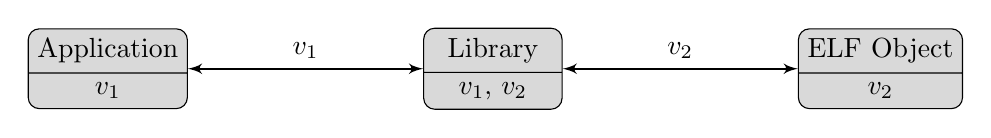
\begin{tikzpicture}[
        >=latex',
        version/.style={
          rectangle split,
          rounded corners,
          minimum width=5em,
          text centered,
          fill=black!15,
          draw,
          rectangle split parts=2,
          node distance=8.5em
        }]
      \node[version] (application) {Application \nodepart{second} $v_1$};
      \node[version] (library) [right=of application] { %
        Library \nodepart{second} $v_1$, $v_2$}
        edge [thick,<->] node[auto,swap] {$v_1$} (application);
      \node[version] (object) [right=of library] { %
        ELF Object \nodepart{second} $v_2$}
        edge [thick,<->] node[auto,swap] {$v_2$} (library);
      \end{tikzpicture}
      \caption{Handling ELF versioning.}\label{fig.versions}
    \end{figure}

    In figure~\vref{fig.versions} the application expects to work with
    ELF specification version $v_1$. The ELF object file conforms to
    ELF specification version $v_2$.  The library understands both
    version $v_1$ and $v_2$ of ELF semantics and so is able to mediate
    between the application and the ELF object.

    In practice, the ELF version has not changed since inception, so
    the current version (\constant{EV\_CURRENT}) is 1.

  \item[\coref{5}] The \function{elf\_begin} function takes an open file
    descriptor and converts it an \type{Elf} handle according to the
    command specified.

    The second parameter to \function{elf\_begin} can be one of
    `\constant{ELF\_C\_READ}' for opening an ELF object for reading,
    `\constant{ELF\_C\_WRITE}' for creating a new ELF object, or
    `\constant{ELF\_C\_RDWR}' for opening an ELF object for updates.
    The mode with which file descriptor \parameter{fd} was opened with
    must be consistent with the this parameter.

    The third parameter to \function{elf\_begin} is only used when
    processing \tool{ar} ar\-chives.  We will look at \tool{ar}
    archive processing in chapter~\vref{chap.ar}.

  \item[\coref{6}] When the ELF library encounters an error, it records
    an error number in an internal location.  This error number may be
    retrieved using the \function{elf\_errno} function.

    The \function{elf\_errmsg} function returns a human readable
    string describing the error number passed in.  As a programming
    convenience, a value of -1 denotes the current error number.

  \item[\coref{3} \coref{7}] The ELF library can operate on \tool{ar}
    archives and ELF objects.  The function \function{elf\_kind}
    returns the kind of object associated with an \type{Elf} handle.
    The return value of the \function{elf\_kind} function is one of
    the values defined by the \type{Elf\_Kind} enumeration in
    \filename{libelf.h}.

  \item[\coref{8}] When you are done with a handle, it is good practice
    to release its resources using the \function{elf\_end} function.
  \end{description}
\end{callout}

Now it is time to get something running.

Save the listing in listing~\vref{src.prog.1} to file
\filename{prog1.c} and then compile and run it as shown in
listing~\vref{scr.prog1}.%
\index{libelf@\library{libelf}!linking with}

\begin{callout}{scr1}
  \begin{lstlisting}[basicstyle=\ttfamily, language={},
      caption=Compiling and running prog1,
      label=scr.prog1]
% cc -o prog1 prog1.c -lelf @\co{1}@
% ./prog1 prog1 @\co{2}@
prog1: elf object
% ./prog1 /usr/lib/libc.a @\co{3}@
/usr/lib/libc.a: ar(1) archive
  \end{lstlisting}

  \begin{description}
  \item[\coref{1}] The \parameter{-lelf} option to the \tool{cc} comand
    informs it to link \tool{prog1} against the \library{libelf}
    library.
  \item[\coref{2}] We invoke \tool{prog1} on itself, and it recognizes
    its own executable as ELF object.  All is well.
  \item[\coref{3}] Here we see that \tool{prog1} recognizes an \tool{ar}
    archive correctly.
  \end{description}
\end{callout}

Congratulations!  You have created your first ELF handling program
using \library{libelf}.

In the next chapter we will look deeper into the ELF format and learn
how to pick an ELF object apart into its component pieces.

\chapter{Peering Inside an ELF Object}\label{chap.peering-inside}

Next, we will look inside an ELF object.  We will look at how an ELF
object is laid out and we will introduce its major parts, namely the
ELF executable header, the ELF program header table and ELF sections.
Along the way we will look at the way \library{libelf} handles
non-native objects.

\section{The Layout of an ELF file}

As an object format, ELF supports multiple kinds of objects:

\begin{itemize}
\item Compilers generate \firstterm{relocatable
  objects}\index{relocatable!definition~of} that contain fragments of
  machine code along with the ``glue'' information needed when
  combining multiple such objects to form a final executable.
\item \firstterm{Executables}\index{executable!definition~of} are programs that are
  in a form that an operating system can launch in a process.  The
  process of forming executables from collections of relocatable
  objects is called \firstterm{linking}\index{linking!definition~of}.
\item \firstterm{Dynamically loadable objects}\index{dynamically
  loadable objects} are those that can be loaded by an executable
  after it has started executing.  Dynamically loadable
  \firstterm{shared libraries}\index{library!shared} are examples of
  such objects.
\end{itemize}

An ELF object consists of a mandatory header named the \firstterm{ELF
  executable header}\index{executable~header}, followed by optional
content in the form of ELF \firstterm{program header table}
\index{program~header!table} and zero or more \firstterm{ELF
  sections}\index{sections} (see figure \vref{fig.elf.layout}).

\begin{figure}
  \caption{The layout of a typical ELF File}\label{fig.elf.layout}
  \begin{center}
    \includegraphics[scale=.75]{fig-elflayout}
  \end{center}
\end{figure}

\begin{itemize}
\item The ELF \firstterm{executable header}\index{executable~header}
  defines the structure of the rest of the file.  This header is
  \emph{always} present in a valid ELF file.  It describes the class
  of the file (whether 32 bit or 64 bit), the type (whether a
  relocatable, executable or shared object), and the byte ordering
  used (little endian or big endian).  It also describes the overall
  layout of the ELF object.  The ELF header is described below.

\item An optional ELF \firstterm{program header table}
  \index{program~header!table} is present in executable objects and
  contains information used by at program load
  time\index{loading!of~programs}.  The program header table is
  described in chapter~\vref{chap.elf-phdr}.

\item The contents of a relocatable ELF object are contained in
  \firstterm{ELF sections}\index{sections}.  These sections are
  described by entries in an \firstterm{ELF section header
    table}\index{sections!header~table}. This table has one entry
  per section present in the file.  Chapter~\vref{chap.elf-sections}
  describes ELF sections and the section header table in further
  detail.
\end{itemize}

Every ELF object is associated with three parameters:

\begin{itemize}
\item Its \firstterm{class}\index{ELF!class} denotes
  whether it is a 32 bit ELF object (\constant{ELFCLASS32}) or a 64
  bit (\constant{ELFCLASS64}) one.
\item Its \firstterm{endianness}\index{ELF!endianness} denotes whether
  it is using little-endian (\constant{ELFDATA2LSB}) or big-endian
  addressing (\constant{ELFDATA2MSB}).
\item Finally, each ELF object is associated with a
  \firstterm{version}\index{ELF!version~number} number as discussed in
  chapter~\vref{chap.getting-started}.
\end{itemize}

These parameters are stored in the ELF executable header.  Let us now
take a closer look at the ELF executable header.

\subsubsection{The ELF Executable Header}\label{sec.ehdr}
Table \vref{src.elf.ehdr} describes the layout of an ELF executable
header using a ``C-like'' notation.%
\index{executable~header!layout}

\begin{callout}{ehdr}
  \begin{table}
    \caption{The ELF Executable Header}\label{src.elf.ehdr}
    \begin{tabular}{rl|l}
      \mbox{} & \tableheader{32 bit Executable Header} &
      \tableheader{64 bit Executable Header} \\ \hline
       & \verb+typedef struct {+&
         \verb+typedef struct {+\\
\co{1} & \verb+  unsigned char e_ident[16];+&
         \verb+  unsigned char e_ident[16];+\\
\co{2} & \verb+  uint16_t      e_type;+&
         \verb+  uint16_t      e_type;+\\
\co{3} & \verb+  uint16_t      e_machine;+&
         \verb+  uint16_t      e_machine;+\\
       & \verb+  uint32_t      e_version;+&
         \verb+  uint32_t      e_version;+\\
       & \verb+  uint32_t      e_entry;+&
         \verb+  uint32_t      e_entry;+\\
\co{4} & \verb+  uint32_t      e_phoff;+&
         \verb+  uint64_t      e_phoff;+\\
\co{5} & \verb+  uint32_t      e_shoff;+&
         \verb+  uint64_t      e_shoff;+\\
       & \verb+  uint32_t      e_flags;+&
         \verb+  uint32_t      e_flags;+\\
       & \verb+  uint16_t      e_ehsize;+&
         \verb+  uint16_t      e_ehsize;+\\
       & \verb+  uint16_t      e_phentsize;+&
         \verb+  uint16_t      e_phentsize;+\\
\co{6} & \verb+  uint16_t      e_phnum;+&
         \verb+  uint16_t      e_phnum;+\\
\co{7} & \verb+  uint16_t      e_shnum;+&
         \verb+  uint16_t      e_shnum;+\\
\co{8} & \verb+  uint16_t      e_shstrndx;+&
         \verb+  uint16_t      e_shstrndx;+\\
       & \verb+} Elf32_Ehdr;+&
         \verb+} Elf64_Ehdr;+\\
    \end{tabular}
  \end{table}

  \begin{description}
  \item[\coref{1}] The first 16 bytes (the \parameter{e\_ident}
    array) contain values that determine the ELF class, version and
    endianness of the rest of the file.  See figure
    \vref{fig.elf.eident}.%
    \index{executable~header!e_ident@\parameter{e\_ident}!definition}

    \begin{figure}[H]
      \caption{The \parameter{e\_ident} array}\label{fig.elf.eident}
      \index{executable~header!e_ident@\parameter{e\_ident} field}
      \begin{center}
        \includegraphics[scale=.9]{fig-eident}
      \end{center}
    \end{figure}

    The first 4 bytes of an ELF object are always 0x7F, `E', `L' and
    `F'.  The next three bytes specify the class of the ELF object
    (\constant{ELFCLASS32} or \constant{ELFCLASS64}), its data
    ordering (\constant{ELFDATA2LSB} or \constant{ELFDATA2MSB}) and
    the ELF version the object conforms to.  With this information on
    hand, the \library{libelf} library can then interpret the rest of
    the ELF executable header correctly.

  \item[\coref{2}] The \parameter{e\_type} member determines the type
    of the ELF object.  For example, it would contain a `1'
    (\constant{ET\_REL}) in a relocatable or `3' (\constant{ET\_DYN})
    in a shared object.%
    \index{executable~header!executable type}

  \item[\coref{3}] The \parameter{e\_machine} member describes the
    machine architecture this ELF object is for.  Example values are `3'
    (\constant{EM\_386}) for the Intel\reg i386\trade architecture and
    `20' (\constant{EM\_PPC}) for the 32-bit PowerPC\trade architecture.%
    \index{executable~header!executable architecture}

  \begin{figure}
    \caption{The ELF Executable Header and Object Layout}
    \label{fig.elf.ehdr-layout}
    \begin{center}
      \includegraphics[scale=.85]{fig-elfhdrlayout}
    \end{center}
  \end{figure}

  \item[\coref{4} \coref{5}] The ELF executable header also describes
    the layout of the rest of the ELF object
    (Figure~\vref{fig.elf.ehdr-layout}). The \parameter{e\_phoff} and
    \parameter{e\_shoff} fields contain the file offsets where the ELF
    program header table and ELF section header table reside.
    These fields are zero if the file does not have a program header
    table or section header table respectively.  The sizes of these
    components are determined by the \parameter{e\_phentsize} and
    \parameter{e\_shentsize} members respectively in conjunction with
    the number of entries in these tables.%
    \index{sections!header~table!layout in file}%
    \index{sections!header~table!entry size}%
    \index{program~header!layout in file}%
    \index{program~header!entry size}

    The ELF executable header describes its own size (in bytes) in
    field \parameter{e\_ehsize}.%
    \index{executable~header!own size}

  \item[\coref{6} \coref{7}] The \parameter{e\_phnum} and
    \parameter{e\_shnum} fields usually contain the number of ELF
    program header table entries and section header table entries.
    Note that these fields are only 2 bytes wide, so if an ELF object
    has a large number of sections or program header table entries,
    then a scheme known as \firstterm{Extended Numbering}%
    \index{extended~numbering} (section~\vref{sec.extended-numbering})
    is used to encode the actual number of sections or program header
    table entries.  When extended numbering is in use these fields
    will contain ``magic numbers'' instead of actual counts.

  \item[\coref{8}] If the ELF object contains sections, then we need a
    way to get at the names of sections.  Section names are stored in
    a string table. The \parameter{e\_shstrndx} stores the section
    index of this string table (see \vref{sec.extended-numbering}) so
    that processing tools know which string table to use for
    retrieving the names of sections.  We will cover ELF string tables
    in more detail in section~\vref{sec.shdr.strtab}.%
    \index{sections!names!string table}
  \end{description}

  The fields \parameter{e\_entry} and \parameter{e\_flags} are used
  for executables and are placed in the executable header for easy
  access at program load time.  We will not look at them further in
  this tutorial.%
  \index{executable~header!program entry point}%
  \index{executable~header!flags}%
\end{callout}

\subsubsection{ELF Class- and Endianness- Independent Processing}
Now let us look at the way the \library{libelf} API set abstracts out
ELF class and endianness for us.

Imagine that you are writing an ELF processing application that is
going to support processing of non-native binaries (say for a machine
with a different native endianness and word size).  It should be
evident that ELF data structures would have two distinct
representations: \index{object~representation} an
\firstterm{in-memory representation} that follows the rules for the
machine architecture that the application running on, and an
\firstterm{in-file representation} that corresponds to the target
architecture for the ELF object.

The application would like to manipulate data in its native memory
representation. \index{object~representation!in-memory} This memory
representation would conform to the native endianness of the host's
CPU and would conform to the address alignment and structure padding
requirements set by the host's machine architecture.

\index{object~representation!in-file} When this data is written into
the target object it may need to be formatted differently.  For
example, it could be packed differently compared to the ``native''
memory representation and may have to be laid out according a
different set of rules for alignment.  The endianness of the data
in-file could be different from that of the in-memory representation.

\begin{figure}
  \caption{File and Memory Representations}\label{fig.representations}
  \begin{center}
    \includegraphics{fig-filemem}
  \end{center}
\end{figure}

Figure \vref{fig.representations} depicts the relationship between the
file and memory representation of an ELF data structure.  As shown in
the figure, the size of an ELF data structure in the file could be
different from its size in memory.  The alignment restrictions
(\parameter{\%falign} and \parameter{\%malign} in the figure) could be
different.  The byte ordering of the data could be different too.%
\index{object~representation!differences between file and memory}

The ELF(3) and GELF(3) API set can handle the conversion of ELF data
structures to and from their file and memory representations
automatically.  For example, when we read in the ELF executable header
in program~\vref{src.prog.2} below, the \library{libelf} library will
automatically do the necessary byteswapping and alignment adjustments
for us.%
\index{ELF!class!agnostic APIs}%
\index{ELF!data conversion!automatic}%
\index{libelf@\library{libelf}!automatic data conversion}

For applications that desire finer-grain control over the conversion
process, the \function{elf\textit{NN}\_xlatetof} and
\function{elf\textit{NN}\_xlatetom} functions are available.  These
functions will translate data buffers containing ELF data structures
between their memory and file representions.%
\index{ELF!data conversion!application control over}

\subsubsection{Extended numbering}\label{sec.extended-numbering}

\index{extended~numbering}%        
The \parameter{e\_shnum}, \parameter{e\_phnum} and
\parameter{e\_shstrndx} fields of the ELF executable header are only 2
bytes long and are not physically capable of representing numbers
larger than 65535.  For ELF objects with a large number of sections,
we need a different way of encoding section numbers.%
\index{extended~numbering!need for}

ELF objects with such a large number of sections can arise due to the
way GCC copes with C++ templates.  When compiling C++ code which uses
templates, GCC generates many sections with names following the
pattern ``.gnu.linkonce.\textit{name}''.  While each compiled ELF
relocatable object will now contain replicated data, the linker is
expected to treat such sections specially at the final link stage,
discarding all but one of each section.

When extended numbering is in use:

\begin{itemize}
\item The \parameter{e\_shnum} field of the ELF executable header is
  always zero and the true number of sections is stored in the
  \parameter{sh\_size} field of the section header table entry at
  index 0.
\item The \index{extended~numbering!sections} true index of the
  section name string table is stored in field \parameter{sh\_link}
  field of the zeroth entry of the section header table, while the
  \parameter{e\_shstrndx} field of the executable header set to
  \constant{SHN\_XINDEX} (0xFFFF).
\item \index{extended~numbering!program header} For extended
  program header table numbering the scheme is similar, with the
  \parameter{e\_phnum} field of the executable header holding the
  value \constant{PN\_XNUM} (0xFFFF) and the \parameter{sh\_link}
  field of the zeroth section header table holding the actual number
  of program header table entries.
\end{itemize}

An \index{extended~numbering!APIs to use} application may use
the functions \function{elf\_getphdrnum}, \function{elf\_getshdrnum}
and \function{elf\_getshdrstrndx} to retrieve the correct value of
these fields when extended numbering is in use.

\section{Example: Reading an ELF executable header}

We will now look at a small program that will print out the ELF
executable header in an ELF object. For this example we will introduce
the GELF(3) API set.%
\index{GELF}

The ELF(3) API is defined in terms of ELF class-dep\-endent types
(\type{Elf32\_\-Ehdr}, \type{Elf64\_\-Shdr}, etc.) and consequently
has many operations that have both 32- and 64- bit variants.  So, in
order to retrieve an ELF executable header from a 32 bit ELF object we
would need to use the function \function{elf32\_getehdr}, which would
return a pointer to an \type{Elf32\_Ehdr} structure.  For a 64-bit ELF
object, the function we would need to use would be
\function{elf64\_getehdr}, which would return a pointer to an
\type{Elf64\_Ehdr} structure.  This duplication is awkward when you
want to write applications that can transparently process either class
of ELF objects.%
\index{ELF!class!agnostic APIs}

The GELF(3) APIs provide an ELF class independent way of writing ELF
applications.  These functions are defined in terms of ``generic''
types that are large enough to hold the values of their corresponding
32- and 64- bit ELF types.  Further, the GELF(3) APIs always work on
\emph{copies} of ELF data structures thus bypassing the
problem of 32- and 64- bit ELF data structures having incompatible
memory layouts.  You can freely mix calls to GELF(3) and ELF(3)
functions.

The downside of using the GELF(3) APIs is the extra copying and
conversion of data that occurs.  This overhead is usually not
significant to most applications.%
\index{GELF!downsides to}

\begin{callout}{prog2}
  \lstinputlisting[caption=Program 2, label=src.prog.2]{prog2.txt}

  \begin{description}
  \item[\coref{1}] Programs using the GELF(3) API set need to include
    \filename{gelf.h}.%
    \index{libelf@\library{libelf}!header \filename{gelf.h}}

  \item[\coref{2}] The GELF(3) functions always operate on a local
    copies of data structures.  The \type{GElf\_Ehdr} type has fields
    that are large enough to contain values for a 64 bit ELF
    executable header.

  \item[\coref{3}] We retrieve the ELF executable header using
    function \function{gelf\_getehdr}.  This function will translate
    the ELF executable header in the ELF object being read to the
    appropriate in-memory representation for type \type{GElf\_Ehdr}.
    For example, if a 32-bit ELF object is being examined, then the
    values in its executable header would be appropriately converted
    (expanded and/or byteswapped) by this function.%
    \index{executable~header!retrieval of}

  \item[\coref{4}] The \function{gelf\_getclass} function retrieves
    the ELF class of the object being examined.%
    \index{ELF!class!retrieval of}

  \item[\coref{5}] Here we show the use of the
    \function{elf\_getident} function to retrieve the contents of the
    \parameter{e\_ident[]} array from the underlying file.  These
    bytes would also be present in the \parameter{e\_ident} member of
    the \parameter{ehdr} structure.%
    \index{ELF!e_ident@\parameter{e\_ident}!retrieval of}

    We print the first few bytes of the \parameter{e\_ident} field
    of the ELF executable header.

  \item[\coref{6}] Following the \parameter{e\_ident} bytes, we
    print the values of some of the fields of the ELF executable
    header structure.

  \item[\coref{7} \coref{8} \coref{9}] The functions
    \function{elf\_getphdrnum}, \function{elf\_get\-shdrnum} and
    \function{elf\_get\\-shdr\-strndx} described in section
    \vref{sec.extended-numbering} should be used to retrieve the count
    of program header table entries, the number of sections, and the
    section name string table index respectively.  Using these
    functions insulates your application from the quirks of extended
    numbering.%
    \index{extended~numbering!use of APIs}%
    \index{extended~numbering!elf_getphdrnum@\function{elf\_getphdrnum}}%
    \index{extended~numbering!elf_getshdrnum@\function{elf\_getshdrnum}}%
    \index{extended~numbering!elf_getshdrstrndx@\function{elf\_getshdrstrndx}}
  \end{description}
\end{callout}

Save the program in listing~\vref{src.prog.2} to file \filename{prog2.c} and
then compile and run it as shown in listing~\vref{scr.prog2}.%
\index{libelf@\library{libelf}!linking with}

\begin{callout}{scr2}
  \newcommand{\at}{@}
  \begin{lstlisting}[language={}, basicstyle=\small\ttfamily,
      label=scr.prog2, caption=Compiling and Running prog2]
% cc -o prog2 prog2.c -lelf @\co{1}@
% ./prog2 prog2 @\co{2}@
prog2: 64-bit ELF object
    e_ident[0..8]    ['\^?' 7F] ['E' 45] ['L' 4C] ['F' 46] \
    ['\^B' 2] ['\^A' 1] ['\^A' 1] ['\^I' 9] ['\^@\at@' 0]
    e_type           0x2
    e_machine        0x3e
    e_version        0x1
    e_entry          0x400a10
    e_phoff          0x40
    e_shoff          0x16f8
    e_flags          0x0
    e_ehsize         0x40
    e_phentsize      0x38
    e_shentsize      0x40
    (shnum)          0x18
    (shstrndx)       0x15
    (phnum)          0x5
  \end{lstlisting}
  \begin{description}
  \item[\coref{1}] The process for compiling and linking a GELF(3)
    using application is the same as that for ELF(3) programs.

  \item[\coref{2}] We run our program on itself.  This listing in this
    tutorial was generated on an AMD64\trade machine running FreeBSD\trade.
  \end{description}

  You should now run \tool{prog2} on other object files that you have
  lying around.  Try it on a few non-native ELF object files too.
\end{callout}

\chapter{Examining the Program Header Table}\label{chap.elf-phdr}

Before a program on disk can be executed by a processor it needs to
brought into main memory.  This process is conventionally called
``loading''\index{loading!of~programs}.

When loading an ELF object into memory, the operating system views it
as comprising of ``segments''\index{segments}.  Each such segment is a
\index{segments!definition~of} contiguous region of data inside
the ELF object that is associated with a particular protection
characteristic (for example, read-only or read-write) and that gets
placed at a specific virtual memory address.

For example, the FreeBSD\trade operating system expects
executables to have an ``executable'' segment containing code, and a
``data'' segment containing statically initialized data.%
\index{segments!example layout}%
The executable segment would be mapped in with read and execute
permissions and could be shared across multiple processes using the
same ELF executable.  The data segment would be mapped in with read
and write permissions and would be made private to each process.  For
dynamically linked executables, the basic idea of grouping related
parts of an ELF object into contiguous ``segments'' still holds,
though there may be multiple segments of each type per process.

\section{The ELF Program Header Table}

The ELF \firstterm{program header table}\index{program~header!table}
describes the segments present in an ELF file.  The location of the
program header table is described by the \parameter{e\_phoff} field of
the ELF executable header (see section~\vref{sec.ehdr}).  The program
header table is a contiguous array of program header table entries,
one entry per segment.

Figure~\vref{fig.elf.phdr.layout} shows graphically how the fields of
a program header table entry specify the segment's placement in file
and in memory.

\begin{figure}
  \caption{ELF Segment Placement}\label{fig.elf.phdr.layout}
  \index{program~header!table!layout}
  \begin{center}
    \includegraphics[scale=.85]{fig-phdrlayout}
  \end{center}
\end{figure}

The structure of each program header table entry is shown in
table~\vref{src.elf.phdr}.\index{program~header!table!entry}

\begin{callout}{phdr}
  \begin{table}[H]
    \caption{ELF Program Header Table Entries}\label{src.elf.phdr}
    \begin{tabular}{rl|ll}
      \mbox{} & \tableheader{32 bit PHDR Table Entry} &
      \tableheader{64 bit PHDR Table Entry}\\ \hline
       & \verb+typedef struct {+&
         \verb+typedef struct {+\\
\co{1} & \verb+  Elf32_Word    p_type;+&
         \verb+  Elf64_Word    p_type;+&\\
\co{2} & \verb+  Elf32_Off     p_offset;+&
         \verb+  Elf64_Word    p_flags;+&\\
\co{3} & \verb+  Elf32_Addr    p_vaddr;+&
         \verb+  Elf64_Off     p_offset;+&\\
\co{4} & \verb+  Elf32_Addr    p_paddr;+&
         \verb+  Elf64_Addr    p_vaddr;+&\\
\co{5} & \verb+  Elf32_Word    p_filesz;+&
         \verb+  Elf64_Addr    p_paddr;+&\\
\co{6} & \verb+  Elf32_Word    p_memsz;+&
         \verb+  Elf64_Xword   p_filesz;+&\\
\co{7} & \verb+  Elf32_Word    p_flags;+&
         \verb+  Elf64_Xword   p_memsz;+&\\
\co{8} & \verb+  Elf32_Word    p_align;+&
         \verb+  Elf64_Xword   p_align;+&\\
       & \verb+} Elf32_Phdr;+ & \verb+} Elf64_Phdr;+&\\
    \end{tabular}
  \end{table}

  \begin{description}
  \item[\coref{1}] The type of the program header table entry is
    encoded using this field.  It holds one of the \constant{PT\_*}
    constants defined in the system headers.%
    \index{segments!type}

    Examples include:
    \begin{itemize}
    \item A segment of type \constant{PT\_LOAD} is loaded into memory.
    \item A segment of type \constant{PT\_NOTE} contains auxiliary
      information.  For example, core filesuse \constant{PT\_NOTE}
      sections to record the name of the process that dumped core.
    \item A \constant{PT\_PHDR} segment describes the program header
      table itself.
    \end{itemize}

    The ELF specification reserves type values from 0x6000\-0000
    (\constant{PT\_LOOS}) to 0x6FFF\-FFFF (\constant{PT\_HIOS}) for
    OS-private information.  Values from 0x7000\-0000
    (\constant{PT\_LOPROC}) to 0x7FFF\-FFFF (\constant{PT\_HIPROC})
    are similarly reserved for processor-specific information.%
    \index{segments!type!reserved values}

  \item[\coref{2}] The \parameter{p\_offset} field holds the file
    offset in the ELF object to the start of the segment being
    described by this table entry.%
    \index{segments!offset in file}

  \item[\coref{3}] The virtual address this segment should be loaded
    at.%
    \index{segments!virtual address of}

  \item[\coref{4}] The physical address this segment should be loaded
    at.  This field does not apply for userland objects.

  \item[\coref{5}] The number of bytes the segment takes up in the
    file.  This number is zero for segments that do not have data
    associated with them in the file.%
    \index{segments!file size of}

  \item[\coref{6}] The number of bytes the segment takes up in memory.%
    \index{segments!memory size of}

  \item[\coref{7}] Additional flags that specify segment properties.
    For example, flag \constant{PF\_X} specifies that the segment in
    question should be made executable and flag \constant{PF\_W}
    denotes that the segment should be writable.%
    \index{segments!flags}

  \item[\coref{8}] The alignment requirements of the segment both in
    memory and in the file.  This field holds a value that is a power
    of two.%
    \index{segments!aligment of}
  \end{description}
\end{callout}

\textbf{Note}: The careful reader will note that the 32- and 64- bit
\type{Elf\_Phdr} structures are laid out differently in memory.  These
differences are handled for you by the functions in the
\library{libelf} library.

\section{Example: Reading a Program Header Table}

We will now look at a program that will print out the program header
table associated with an ELF object.  We will continue to use the
GELF(3) API set for this example.  The ELF(3) API set also offers two
ELF class-dependent APIs that retrieve the program header table from
an ELF object: \function{elf32\_getphdr} and
\function{elf64\_getphdr}, but these require us to know the ELF class
of the object being handled.%
\index{ELF!class!agnostic APIs}

\begin{callout}{prog3}
  \lstinputlisting[caption=Program 3, label=src.prog.3]{prog3.txt}
  
  \begin{description}
  \item[\coref{1}] We need to include \filename{gelf.h} in order to
    use the GELF(3) APIs.
  \item[\coref{2}] The \type{GElf\_Phdr} type has fields that are
    large enough to contain the values in an \type{Elf32\_Phdr} type
    and an \type{Elf64\_Phdr} type.%
    \index{ELF!class!agnostic APIs}
  \item[\coref{3}] We retrieve the number of program header table
    entries using the function \function{elf\_getphdrnum}.  Note that
    the program header table is optional; for example, an ELF
    relocatable object will not have a program header table.%
    \index{program~header!table!retrieval of}
  \item[\coref{4} \coref{5}] We iterate over all valid indices for the
    object's program header table, retrieving the table entry at each
    index using the \function{gelf\_getphdr} function.%
    \index{program~header!table!iteration over}
  \item[\coref{6} \coref{7}] We then print out the contents of the
    entry so retrieved.  We use a helper function
    \function{print\_ptype} to convert the \parameter{p\_type} member
    to a readable string.
  \end{description}
\end{callout}

Save the program in listing~\vref{src.prog.3} to file \filename{prog3.c} and
then compile and run it as shown in listing~\vref{scr.prog3}.%
\index{libelf@\library{libelf}!linking with}

\begin{callout}{scr3}
  \begin{lstlisting}[language={}, basicstyle=\small\ttfamily,
      label=scr.prog3, caption=Compiling and Running prog3]
% cc -o prog3 prog3.c -lelf @\co{1}@
% ./prog3 prog3 @\co{2}@
PHDR 0:
    p_type               0x6 "PHDR" @\co{3}@
    p_offset             0x34
    p_vaddr              0x8048034
    p_paddr              0x8048034
    p_filesz             0xc0
    p_memsz              0xc0
    p_flags              0x5 [ execute read ]
    p_align              0x4
PHDR 1:
    p_type               0x3 "INTERP" @\co{4}@
    p_offset             0xf4
    p_vaddr              0x80480f4
    p_paddr              0x80480f4
    p_filesz             0x15
    p_memsz              0x15
    p_flags              0x4 [ read ]
    p_align              0x1
PHDR 2:
    p_type               0x1 "LOAD" @\co{5}@
    p_offset             0x0
    p_vaddr              0x8048000
    p_paddr              0x8048000
    p_filesz             0xe67
    p_memsz              0xe67
    p_flags              0x5 [ execute read ]
    p_align              0x1000
PHDR 3:
    p_type               0x1 "LOAD" @\co{6}@
    p_offset             0xe68
    p_vaddr              0x8049e68
    p_paddr              0x8049e68
    p_filesz             0x11c
    p_memsz              0x13c
    p_flags              0x6 [ read write ]
    p_align              0x1000
PHDR 4:
    p_type               0x2 "DYNAMIC"
    p_offset             0xe78
    p_vaddr              0x8049e78
    p_paddr              0x8049e78
    p_filesz             0xb8
    p_memsz              0xb8
    p_flags              0x6 [ read write ]
    p_align              0x4
PHDR 5:
    p_type               0x4 "NOTE"
    p_offset             0x10c
    p_vaddr              0x804810c
    p_paddr              0x804810c
    p_filesz             0x18
    p_memsz              0x18
    p_flags              0x4 [ read ]
    p_align              0x4
  \end{lstlisting}

  \begin{description}
  \item[\coref{1}] Compile and link the program in the standard way.
  \item[\coref{2}] We make our program examine its own program header
    table.  This listing was generated on an i386\trade machine
    running FreeBSD\trade.
  \item[\coref{3}] The very first entry in this program header table
    describes the program header table itself.%
    \index{program~header!table!self-description}
  \item[\coref{4}] An entry of type \constant{PT\_INTERP} is used to
    point the kernel to the ``interpreter'' associated with this ELF
    object.  This is usually a runtime loader, such as
    \filename{/libexec/ld-elf.so.1}.
  \item[\coref{5} \coref{6}] This object has two loadable segments:
    one with execute and read permissions and one with read and write
    permissions.  Both these segments require page alignment.%
    \index{segments!examples of}
  \end{description}
\end{callout}

You should now run \tool{prog3} on other object files.

\begin{itemize}
\item Try a relocatable object file created by a \tool{cc -c}
  invocation.  Does it have an program header table?
\item Try \tool{prog3} on shared libraries.  What do their program
  header tables look like?
\item Can you locate ELF objects on your system that have
  \constant{PT\_TLS} header entries?
\end{itemize}

\chapter{Looking at Sections}\label{chap.elf-sections}

In the previous chapter we looked at the way an executable ELF objects
are viewed by the operating system.  In this section we will look at
the features of the ELF format that are used by compilers and linkers.

For linking, data in an ELF object is grouped into
\firstterm{sections}\index{sections}.  Each ELF section represents
one kind of data.  For example, a section could contain a table of
strings used for program symbols, another could contain debug
information, and another could contain machine code.  Non-empty
sections do not overlap in the file.%
\index{sections!use of}

ELF sections are described by entries in an \firstterm{ELF section
  header table}\index{sections!header~table}.  This table is
usually placed at the very end of the ELF object (see
figure~\vref{fig.elf.layout}).  Table~\vref{src.elf.shdr} describes
the elements of section header table entry and
figure~\vref{fig.elf.shdrlayout} shows graphically how the fields of
an ELF section header specify the section's placement.%
\index{sections!placement in file}

\begin{callout}{shdr}
  \begin{table}[H]
    \caption{ELF Section Header Table Entries}\label{src.elf.shdr}
    \begin{tabular}{rl|l}
      \mbox{} & \tableheader{32 bit SHDR Table Entry} &
      \tableheader{64 bit SHDR Table Entry} \\ \hline
       & \verb+typedef struct {+ & \verb+typedef struct {+ \\
\co{1} & \verb+  Elf32_Word   sh_name;+&
         \verb+  Elf64_Word   sh_name;+\\
\co{2} & \verb+  Elf32_Word   sh_type;+&
         \verb+  Elf64_Word   sh_type;+\\
\co{3} & \verb+  Elf32_Xword  sh_flags;+&
         \verb+  Elf64_Xword  sh_flags;+\\
       & \verb+  Elf32_Addr   sh_addr;+&
         \verb+  Elf64_Addr   sh_addr;+\\
       & \verb+  Elf32_Off    sh_offset;+&
         \verb+  Elf64_Off    sh_offset;+\\
\co{4} & \verb+  Elf32_Xword  sh_size;+&
         \verb+  Elf64_Xword  sh_size;+\\
\co{5} & \verb+  Elf32_Word   sh_link;+&
         \verb+  Elf64_Word   sh_link;+\\
\co{6} & \verb+  Elf32_Word   sh_info;+&
         \verb+  Elf64_Word   sh_info;+\\
\co{7} & \verb+  Elf32_Word   sh_addralign;+&
         \verb+  Elf64_Word   sh_addralign;+\\
\co{8} & \verb+  Elf32_Word   sh_entsize;+&
         \verb+  Elf64_Word   sh_entsize;+\\
       & \verb+} Elf32_Shdr;+ & \verb+} Elf64_Shdr;+ \\
    \end{tabular}
  \end{table}

  \begin{description}
  \item[\coref{1}] The \parameter{sh\_name} field is used to encode a
    section's name.  As section names are variable length strings,
    they are not kept in the section header table entry itself.%
    \index{sections!names!representation of}%
    Instead, all section names are collected into an object-wide
    string table holding section names and the \parameter{sh\_name}
    field of each section header stores an \emph{index} into the
    string table.  The ELF executable header has an
    \parameter{e\_shstrndx} member that points to the section index of
    this string table.%
    \index{sections!names!string table}
    ELF string tables, and the way to read them programmatically are
    described in section~\vref{sec.shdr.strtab}.

  \item[\coref{2}] The \parameter{sh\_type} field specifies the
    section type.  Section types are defined by the \constant{SHT\_*}
    constants defined in the system's ELF headers.  For example, a
    section of type \constant{SHT\_PROGBITS} is defined to contain
    executable code, while a section type \constant{SHT\_SYMTAB}
    denotes a section containing a symbol table.%
    \index{sections!type}

    The ELF specification reserves values in the range 0x6000\-0000 to
    0x6FFF\-FFFF to denote OS-specific section types, and values in the
    range 0x7000\-0000 to 0x7FFF\-FFFF for processor-specific section
    types.  In addition, applications have been given the range
    0x80000000 to 0xFFFFFFFF for their own use.%
    \index{sections!type!reserved values}

  \item[\coref{3}] Section flags indicate whether a section has
    specific properties, e.g., whether it contains writable data or
    instructions, or whether it has special link ordering
    requirements.  Flag values from 0x00100000 to 0x08000000 (8 flags)
    are reserved for OS-specific uses.  Flags values from 0x10000000
    to 0x80000000 (4 flags) are reserved for processor specific uses.%
    \index{sections!flags}

  \item[\coref{4}] The \parameter{sh\_size} member specifies the size
    of the section in bytes.%
    \index{sections!size of}

  \item[\coref{5} \coref{6}] The \parameter{sh\_link} and
    \parameter{sh\_info} fields contain additional additional section
    specific information.  These fields are described in the elf(5)
    manual page.

  \item[\coref{7}] For sections that have specific alignment
    requirements, the \parameter{sh\_addralign} member holds the
    required alignment.  Its value is a power of two.%
    \index{sections!alignment of}

  \item[\coref{8}] For sections that contain arrays of fixed-size
    elements, the \parameter{sh\_entsize} member specifies the size of
    each element.%
    \index{sections!entry sizes}
  \end{description}
\end{callout}

\begin{figure}
  \begin{center}
    \includegraphics[scale=.85]{fig-shdrlayout}
  \end{center}
  \caption{Section layout}\label{fig.elf.shdrlayout}
\end{figure}

There are a couple of other quirks associated with ELF sections. Valid
section indices range from \constant{SHN\_UNDEF} (0) upto but not
including \constant{SHN\_LORESERVE} (0xFF00).  Section indices between
0xFF00 and 0xFFFF are used to denote special sections (like FORTRAN
COMMON blocks).  Thus if an ELF file has more than 65279 (0xFEFF)
sections, then it needs to use extended section numbering (see
section~\vref{sec.extended-numbering}).%
\index{sections!indices!valid indices}

The section header table entry at index `0' (\constant{SHN\_UNDEF}) is
treated specially: it is always of type \constant{SHT\_NULL}.  It has
its members set to zero except when extended numbering is in use, see
section~\vref{sec.extended-numbering}.%
\index{sections!indices!SHN_UNDEF@\constant{SHN\_UNDEF}}

\section{ELF section handling with \library{libelf}}

You can conveniently retrieve the contents of sections and section
headers using the APIs in the ELF(3) library.  Function
\function{elf\_getscn} will retrieve section information for a
requested section number.%
\index{sections!retrieval!elf_getscn@\function{elf\_getscn}}%
Iteration through the sections of an ELF
file is possible using function \function{elf\_nextscn}.%
\index{sections!iteration through!elf_nextscn@\function{elf\_nextscn}}%
These routines will take care of translating between in-file and in-memory
representations, thus simplifying your application.%
\index{object~representation!automatic translation}

In the ELF(3) API set, ELF sections are managed using \type{Elf\_Scn}
descriptors.  There is one \type{Elf\_Scn} descriptor per ELF section
in the ELF object.  Functions \function{elf\_getscn} and
\function{elf\_nextscn} retrieve pointers to \type{Elf\_Scn}
descriptors for pre-existing sections in the ELF object.  (Chapter
\vref{chap.creating-elf} covers the use of function
\function{elf\_newscn} for allocating new sections).%
\index{Elf_Scn@\type{Elf\_Scn}!use of}.

Given an \type{Elf\_Scn} descriptor, functions
\function{elf32\_\-getshdr} and \function{elf64\_\-getshdr} retrieve
its associated section header table entry.  The GELF(3) API set offers
an equivalent ELF-class independent function \function{gelf\_getshdr}.%
\index{ELF!class!agnostic APIs}%
\index{sections!header table entry!retrieval of}%
\index{sections!header table entry!elf32_getshdr@\function{elf32\_getshdr}}%
\index{sections!header table entry!elf64_getshdr@\function{elf64\_getshdr}}%
\index{sections!header table entry!gelf_getshdr@\function{gelf\_getshdr}}

Each \type{Elf\_Scn} descriptor can be associated with zero or more
\type{Elf\_Data} descriptors.  \type{Elf\_Data} descriptors describe
regions of application memory that contain the actual data in the ELF
section.  \type{Elf\_Data} descriptors for a given \type{Elf\_Scn}
descriptor are retrieved using the \function{elf\_getdata} function.%
\index{Elf_Scn@\type{Elf\_Scn}!Elf_Data descriptors@\type{Elf\_Data} descriptors}

Figure~\vref{fig.elf.scn} shows graphically how an \type{Elf\_Scn}
descriptor could conceptually cover the content of a section with
\type{Elf\_Data} descriptors.%
\index{sections!coverage by data descriptors}

\begin{figure}
  \begin{center}
    \includegraphics{fig-scn}
  \end{center}
  \caption{Managing data in an Elf Section}\label{fig.elf.scn}
\end{figure}

Figure~\vref{fig.elf.data} depicts how an \type{Elf\_Data} structure
describes a chunk of application memory.  Note that the figure
reflects the fact that the in-memory representation of data could have
a different size and endianness than its in-file
representation.%
\index{Elf_Data@\type{Elf\_Data}!describing application memory}

\begin{figure}
  \begin{center}
    \includegraphics{fig-data}
  \end{center}
  \caption{\type{Elf\_Data} descriptors}\label{fig.elf.data}
\end{figure}

Figure~\vref{fig.elf.scn-data.decl} shows the C definition of the
\type{Elf\_Scn} \index{Elf_Scn@\type{Elf\_Scn}!definition~of} and
\type{Elf\_Data} \index{Elf_Data@\type{Elf\_Data}!definition~of}
descriptors.

\begin{callout}{data}
  \begin{lstlisting}[caption=Definition of Elf\_Data and Elf\_Scn,
      label=fig.elf.scn-data.decl, basicstyle=\small\ttfamily]
typedef struct _Elf_Scn Elf_Scn;   @\co{1}@ 
typedef struct _Elf_Data {
        /*
         * `Public' members that are part of the ELF(3) API.
         */
        uint64_t        d_align;   @\co{2}@
        void            *d_buf;    @\co{3}@
        uint64_t        d_off;     @\co{4}@
        uint64_t        d_size;    @\co{5}@
        Elf_Type        d_type;    @\co{6}@
        unsigned int    d_version; @\co{7}@
        /* ... other library-private fields ... */
} Elf_Data;
  \end{lstlisting}

  \begin{description}
  \item[\coref{1}] The \type{Elf\_Scn} type is opaque to the
    application.
  \item[\coref{2}] The \parameter{d\_align} member specifies alignment
    of data referenced in the \type{Elf\_Data} with respect to its
    containing section.%
    \index{Elf_Data@\type{Elf\_Data}!alignment}
  \item[\coref{3}] The \parameter{d\_buf} member points to a contiguous
    region of memory holding data.%
    \index{Elf_Data@\type{Elf\_Data}!data pointer}
  \item[\coref{4}] The \parameter{d\_off} member contains the file
    offset \emph{from the start of the section} of the data in this
    buffer.  This field is usually managed by the library, but is
    under application control if the application has requested full
    control of the ELF file's layout (see
    chapter~\vref{chap.creating-elf}).%
    \index{Elf_Data@\type{Elf\_Data}!offset in section}
  \item[\coref{5}] The \parameter{d\_size} member contains the size of
    the memory buffer.%
    \index{Elf_Data@\type{Elf\_Data}!data size}
  \item[\coref{6}] The \parameter{d\_type} member specifies the ELF
    type of the data contained in the data buffer.  Legal values for
    this member are precisely those defined by the \type{Elf\_Type}
    enumeration in \filename{libelf.h}.%
    \index{Elf_Data@\type{Elf\_Data}!data type}
  \item[\coref{7}] The \parameter{d\_version} member specifies the
    working version for the data in this descriptor.  It must be one
    of the values supported by the \library{libelf} library.%
    \index{Elf_Data@\type{Elf\_Data}!descriptor version}
  \end{description}
\end{callout}

Before we look at an example program we need to understand how string
tables are implemented by \library{libelf}.

\subsection{String Tables}\label{sec.shdr.strtab}

String tables hold variable length strings, allowing other structures
in an ELF object to refer to strings using offsets into the string
table.  Sections containing string tables have type
\constant{SHT\_STRTAB}.%
\index{sections!string~table}

\begin{figure}
  \begin{center}
    \includegraphics[scale=.9]{fig-strtab}
  \end{center}
  \caption{String Table Layout}\label{fig.elf.strtab}
\end{figure}

Figure~\vref{fig.elf.strtab} shows the layout of a string table
graphically:%
\index{sections!string~table!layout}

\begin{itemize}
\item The initial byte of a string table is \constant{NUL} (a
  `\(\backslash\)0').  This allows an string offset value of zero to
  denote the NULL string.
\item Subsequent strings are separated by \constant{NUL} bytes.
\item The final byte in the section is again a \constant{NUL} so as to
  terminate the last string in the string table.
\end{itemize}

An ELF file can have multiple string tables; for example, section
names could be kept in one string table and symbol names in another.

Given the section index of a section containing a string table,
applications would use the \function{elf\_strptr} function to convert
a string offset to \type{char *} pointer usable by C code.%
\index{sections!string~table!retrieval of strings}%
\index{sections!string~table!elf_strptr@\function{elf\_strptr}}

\section{Example: Listing section names}

Let us now write a program that would retrieve and print the names of
the sections present in an ELF object.  This example will show you how
to use:
\begin{itemize}
\item Functions \function{elf\_nextscn} and \function{elf\_getscn} to
  retrieve \type{Elf\_Scn} descriptors.
\item Function \function{gelf\_getshdr} to retrieve a section header
  table entry corresponding to a section descriptor.%
  \index{ELF!class!agnostic APIs}
\item Function \function{elf\_strptr} to convert section name indices
  to NUL-terminated strings.%
  \index{sections!names!retrieval of}
\item Function \function{elf\_getdata} to retrieve translated data
  associated with a section.%
  \index{sections!data!retrieval of}
\end{itemize}

\begin{callout}{prog4}
  \lstinputlisting[caption=Program 4, label=src.prog.4]{prog4.txt}

  \begin{description}
    \item[\coref{1}] We retrieve the section index of the ELF section
      containing the string table of section names using function
      \function{elf\_getshdrstrndx}.  The use of
      \function{elf\_getshdrstrndx} allows our program to work
      correctly when the object being examined has a very large number
      of sections.%
      \index{sections!names!string table}
    \item[\coref{2}] Function \function{elf\_nextscn} has the useful
      property that it returns the pointer to section number `1' if a
      NULL section pointer is passed in.  Recall that section number `0'
      is always of type \constant{SHT\_NULL} and is not interesting to
      applications.
    \item[\coref{3}] We loop over all sections in the ELF object.
      Function \function{elf\_nextscn} will return NULL at the end,
      which is a convenient way to exit the processing loop.
    \item[\coref{4}] Given a \type{Elf\_Scn} pointer, we retrieve the
      associated section header using function
      \function{gelf\_getshdr}.  The \parameter{sh\_name} member of
      this structure holds the required offset into the section name
      string table.%
      index{sections!header table entry!retrieval of}
    \item[\coref{5}] We convert the string offset in member
      \parameter{sh\_name} to a \type{char *} pointer using function
      \function{elf\_strptr}.  This value is then printed using
      \function{printf}.%
      \index{sections!names!retrieval of}%
      \index{sections!names!elf_strptr@\function{elf\_strptr}}%
    \item[\coref{6}] We retrieve the section descriptor associate with
      the string table holding section names.  Variable
      \parameter{shstrndx} was retrieved by a prior call to function
      \function{elf\_getshdrstrndx}.%
      \index{sections!names!string table}
    \item[\coref{7}] We cycle through the \type{Elf\_Data} descriptors
      associated with the section in question, printing the characters
      in each data buffer.
  \end{description}
\end{callout}

Save the program in listing~\vref{src.prog.4} to file
\filename{prog4.c} and then compile and run it as shown in
listing~\vref{scr.prog4}.%
\index{libelf@\library{libelf}!linking with}

\begin{callout}{scr4}
  \newcommand{\at}{@}
  \begin{lstlisting}[language={}, basicstyle=\small\ttfamily,
      label=scr.prog4, caption=Compiling and Running prog4]
% cc -o prog4 prog4.c -lelf @\co{1}@
% ./prog4 prog4 @\co{2}@
Section 0001 .interp
Section 0002 .note.ABI-tag
Section 0003 .hash
Section 0004 .dynsym
Section 0005 .dynstr
Section 0006 .rela.plt
Section 0007 .init
Section 0008 .plt
Section 0009 .text
Section 0010 .fini
Section 0011 .rodata
Section 0012 .data
Section 0013 .eh_frame
Section 0014 .dynamic
Section 0015 .ctors
Section 0016 .dtors
Section 0017 .jcr
Section 0018 .got
Section 0019 .bss
Section 0020 .comment
Section 0021 .shstrtab @\co{3}@
Section 0022 .symtab
Section 0023 .strtab
.shstrab: size=287 @\co{4}@
\^@\at@ . s y m t a b \^@\at@ . s t r t a b
\^@\at@ . s h s t r t a b \^@\at@ . i n t e
r p \^@\at@ . h a s h \^@\at@ . d y n s y m
@\ldots{}\textit{etc}\ldots@
  \end{lstlisting}

  \begin{description}
  \item[\coref{1}] Compile and link the program in the standard way.
  \item[\coref{2}] We make our program print the names of its own
    sections.
  \item[\coref{3}] One of the sections contains the string table used
    for sections names themselves.  This section is called
    \parameter{.shstrtab} by convention.
  \item[\coref{4}] This is the content of the string table holding
    section names.
  \end{description}
\end{callout}

\chapter{Creating new ELF objects}\label{chap.creating-elf}

We will now look at how ELF objects can be created (and modified, see
section~\vref{sec.modifying-elf}) using the \library{libelf}
library.\index{ELF!creation~of}

Broadly speaking, the steps involved in creating an ELF file with
\library{libelf} are:
\begin{enumerate}
\item An ELF descriptor needs to be allocated with a call to
  \function{elf\_begin}, passing in the parameter
  \constant{ELF\_C\_WRITE}.%
  \index{ELF!descriptor!allocation}%

\item You would then allocate an ELF executable header using one of
  the \function{elf32\_newehdr}, \function{elf64\_newehdr} or
  \function{gelf\_newehdr} functions.  Note that this is a mandatory
  step since an ELF executable header is always present in an ELF
  object.  The ELF ``class'', of the object, i.e., whether the object
  is a 32-bit or 64-bit one, is fixed at this time.%
  \index{executable~header!allocation!functions}%
  \index{executable~header!allocation!gelf_newehdr@\function{gelf\_newehdr}}%
\item An ELF program header table is optional and can be allocated
  using one of functions \function{elf32\_newphdr},
  \function{elf64\_newphdr} or \function{gelf\_newphdr}.  The program
  header table can be allocated anytime after the executable header
  has been allocated.%
  \index{program~header!table!allocation of}
\item Sections may be added to an ELF object using function
  \function{elf\_newscn}.  \type{Elf\_Data} descriptors associated
  with an ELF section can be added to a section descriptor using
  function \function{elf\_newdata}. ELF sections can be allocated
  anytime after the object's executable header has been allocated.%
  \index{sections!adding to an object}%
  \index{Elf_Data@\type{Elf\_Data}!adding to section descriptor}
\item If you are creating an ELF object for a non-native architecture,
  you can change the byte ordering of the object by changing the byte
  order byte at offset \constant{EI\_DATA} in the ELF header.%
  \index{object~creation!non-native byte order}
\item Once your data is in place, you then ask the \library{libelf}
  library to write out the final ELF object using function
  \function{elf\_update}.%
  \index{executable~header!updating!with \function{elf\_update}}
\item Finally, you close the ELF descriptor allocated using function
  \function{elf\_end}.
\end{enumerate}

\section{Example: Creating an ELF object}

In listing~\vref{src.prog.5} we will look at a program that creates a
simple ELF object with a program header table, one ELF section
containing translatable data and one ELF section containing a section
name string table.  We will mark the ELF of the object as using a
32-bit, MSB-first data ordering.

\begin{callout}{prog5}
  \lstinputlisting[caption=Program 5, label=src.prog.5]{prog5.txt}

  \begin{description}
  \item[\coref{1}] We include \filename{libelf.h} to bring in
    prototypes for \library{libelf}'s functions.
    \item[\coref{2}] We will create an ELF section containing `hash'
      values.  These values are present in host-native order in the
      array \parameter{hash\_words}.  These values will be translated
      to the appropriate byte order by the \library{libelf} library
      when the object file is created.%
      \index{sections!hash~values}
    \item[\coref{3}] We use a pre-fabricated ELF string table to hold
      section names.  See section~\vref{sec.shdr.strtab} for more
      information on the layout of ELF string tables.%
      \index{sections!string~table}
    \item[\coref{4}] The first step to create an ELF object is to
      obtain a file descriptor from the OS that is opened for writing.
    \item[\coref{5}] By passing parameter \constant{ELF\_C\_WRITE} to
      function \function{elf\_begin}, we obtain an ELF descriptor
      suitable for creating new ELF objects.%
      \index{object~creation!with \function{elf\_begin}}
    \item[\coref{6}] We allocate an ELF executable header and set the
      \constant{EI\_DATA} byte in its \parameter{e\_ident} member.
      The machine type is set to \constant{EM\_PPC} denoting the
      PowerPC architecture, and the object is marked as an ELF
      executable.%
      \index{executable~header!allocation}
    \item[\coref{7}] We allocate an ELF program header table with one
      entry.  At this point of time we do not know how the ELF object
      will be laid out so we don't know where the ELF program header
      table will reside.  We will update this entry later.
    \item[\coref{8}] We create a section descriptor for the section
      containing the `hash' values, and associate the data in the
      \parameter{hash\_words} array with this descriptor.  The type of
      the section is set to \constant{SHT\_HASH}.  The library will
      compute its size and location in the final object and will
      byte-swap the values when creating the ELF object.
    \item[\coref{9}] We allocate another section for holding the
      string table.  We use the pre-fabricated string table in
      variable \parameter{string\_table}.  The type of the section is
      set to \constant{SHT\_STRTAB}.  Its offset and size in the file
      will be computed by the library.%
      index{sections!string~table!allocation~of}
    \item[\coref{10}] We set the string table index field in the ELF
      executable header using the function
      \function{elf\_setshstrndx}.%
      \index{executable~header!setting the string table index}
    \item[\coref{11}] Calling function \function{elf\_update} with
      parameter \constant{ELF\_C\_NULL} indicates that the
      \library{libelf} library is to compute the layout of the object,
      updating all internal data structures, but \emph{not} write it
      out.  We can thus fill in the values in the ELF program header
      table entry that we had allocated using the new values in the
      executable header after this call to \function{elf\_update}.
      The program header table is then marked ``dirty'' using a call
      to function \function{elf\_flagdata}, so that a subsequent call
      to \function{elf\_update} will use the new contents.%
      \index{executable~header!updating!with \function{elf\_update}}
    \item[\coref{12}] A call to function \function{elf\_update} with
      parameter \constant{ELF\_C\_WRITE} causes the object file to be
      written out.%
      \index{object~creation!writing to file!with \function{elf\_update}}
  \end{description}
\end{callout}

Save the program in listing~\vref{src.prog.5} to file
\filename{prog5.c} and then compile and run it as shown in
listing~\vref{scr.prog5}.%
\index{libelf@\library{libelf}!linking with}

\begin{callout}{scr5}
  \begin{lstlisting}[language={}, basicstyle=\small\ttfamily,
      label=scr.prog5, caption=Compiling and Running prog5]
% cc -o prog5 prog5.c -lelf @\co{1}@
% ./prog5 foo
% file foo @\co{2}@
foo: ELF 32-bit MSB executable, PowerPC or cisco 4500, \
     version 1 (SYSV), statically linked, stripped
% readelf -a foo @\co{3}@
ELF Header:
  Magic:   7f 45 4c 46 01 02 01 00 00 00 00 00 00 00 00 00
  Class:                             ELF32
  Data:                              2's@\,@complement,@\,@big@\,@endian
  Version:                           1 (current)
  OS/ABI:                            UNIX - System V
  ABI Version:                       0
  Type:                              EXEC (Executable file)
  Machine:                           PowerPC
  Version:                           0x1
  Entry point address:               0x0
  Start of program headers:          52 (bytes into file)
  Start of section headers:          112 (bytes into file)
  Flags:                             0x0
  Size of this header:               52 (bytes)
  Size of program headers:           32 (bytes)
  Number of program headers:         1
  Size of section headers:           40 (bytes)
  Number of section headers:         3
  Section header string table index: 2
@\ldots etc\ldots@
  \end{lstlisting}

  \begin{description}
  \item[\coref{1}] Compile, link and run the program in the standard
    way.
  \item[\coref{2} \coref{3}] We use the \tool{file} and \tool{readelf}
    programs to examine the object that we have created.
  \end{description}
\end{callout}

\section{The finer points in creating ELF objects}

Some of the finer points in creating ELF objects using the
\library{libelf} library are examined below.  We cover memory
management rules, ELF data structure lifetimes, and how an application
can take full control over an object's layout.  We also briefly cover
how to modify an existing ELF object.

\subsection{Controlling ELF Layout}
By default, the \library{libelf} library will lay out your ELF objects
for you.  The default layout is shown in figure~\vref{fig.elf.layout}.%
\index{object~creation!default~layout}%
An application may request fine-grained control over the ELF object's
layout by setting the flag \constant{ELF\_F\_LAYOUT} on the ELF
descriptor using function \function{elf\_flagelf}.%
\index{object~creation!layout!application~control~of}

Once an ELF descriptor has been flagged with flag
\constant{ELF\_F\_LAYOUT} the following members of the ELF data
structures come under application control:

\begin{itemize}
\item The \parameter{e\_phoff} and \parameter{e\_shoff} fields, which
  determine whether the ELF program header table and section header
  table start.
\item For each section, the \parameter{sh\_addralign},
  \parameter{sh\_offset}, and \parameter{sh\_size} fields in its
  section header.
\end{itemize}

These fields must set prior to calling function
\function{elf\_update}.

The library will fill ``gaps'' between parts of the ELF file with a
\firstterm{fill character}\index{ELF!fill character}.  An application
may set the fill character using the function \function{elf\_fill}.
The default fill character is a zero byte.%
\index{object~creation!layout!fill~character}%
\index{object~creation!layout!elf_fill@\function{elf\_fill}}

\subsection{Memory Management}

Applications pass pointers to allocated memory to the \library{libelf}
library by setting the \parameter{d\_buf} members of \type{Elf\_Data}
structures passed to the library.  The \library{libelf} library also
passes data back to the application using the same mechanism.  In
order to keep tracking memory ownership simple, the \library{libelf}
library follows the rule that it will never attempt to free data that
it did not allocate.  Conversely, the application is also not to free
memory allocated by the \library{libelf} library.%
\index{object~creation!memory~management~rules}

\subsection{\library{libelf} data structure lifetimes}
As part of the process of writing out an ELF object, the
\library{libelf} library may release or reallocate its internal
bookkeeping structures.

A rule to be followed when using the \library{libelf} library is that
all pointers to returned data structures (e.g., pointers to
\type{Elf\_Scn} and \type{Elf\_Data} structures or to other ELF
headers \emph{become invalid} after a call to function
\function{elf\_update} with parameter \constant{ELF\_C\_WRITE}.

After a successful call to function \function{elf\_update} all ELF
data structures will need to be retrieved afresh.%
\index{object~creation!refreshing of data structures}

\subsection{Modifying existing ELF objects}\label{sec.modifying-elf}

The \library{libelf} library also allows existing ELF objects to be
modified.  The process is similar to that for creating ELF objects,
the differences being:%
\index{object~modification!process to follow}

\begin{itemize}
\item The underlying file object would need to be opened for reading
  and writing, and the call to function \function{elf\_begin} would
  use parameter \constant{ELF\_C\_RDWR} instead of
  \constant{ELF\_C\_WRITE}.
\item The application would use the \function{elf\_get*} APIs to
  retrieve existing ELF data structures in addition to the
  \function{elf\_new*} APIs used for allocating new data structures.
  The \library{libelf} library would be informed of modifications to
  ELF data structures by calls to the appropriate
  \function{elf\_flag*} functions.%
  \index{object~modification!flagging modified data}
\end{itemize}

The rest of the program flow would be similar to the object creation
case.

\chapter{Processing ar(1) archives}\label{chap.ar}

The \library{libelf} library also offers support for reading archives
members in an ar(1) archive.  This support is ``read-only''; you
cannot create new ar(1) archives or update members in an archive using
these functions.  The \library{libelf} library supports both random
and sequential access to the members of an ar(1) archive.

\section{Archive structure}

Each ar(1) archive starts with a sequence of 8 signature bytes (see
the constant \constant{ARMAG}\index{ar~archive!magic} defined in the
system header \filename{ar.h}).  The members of the archive follow,
each member preceded by an \firstterm{archive
  header}\index{ar~archive!header} describing the metadata associated
with the member.  Figure~\vref{fig.arstr} depicts the structure of an
ar(1) archive pictorially.

\begin{figure}
  \begin{center}
    \includegraphics[scale=.9]{fig-arstr}
  \end{center}
  \caption{The structure of ar(1) archives}\label{fig.arstr}
\end{figure}

Each archive header is a collection of fixed size ASCII
strings.\index{ar~archive!header!layout} Archive headers are required
to reside at even offsets in the archive file.
Figure~\vref{src.arhdr} shows the layout of the archive header as a C
structure.

\begin{lstlisting}[caption=Archive Header Layout, label=src.arhdr]
struct ar_hdr {
    char ar_name[16]; /* file name */
    char ar_date[12]; /* file modification time */
    char ar_uid[6];   /* creator user id */
    char ar_gid[6];   /* creator group id */
    char ar_mode[8];  /* octal file permissions */
    char ar_size[10]; /* size in bytes */
#define        ARFMAG   "`\n"
    char ar_fmag[2];  /* consistency check */
} __packed;
\end{lstlisting}

The initial members of an ar(1); archive may be special:

\begin{itemize}
\item An archive member with name ``/'' is an \firstterm{archive
  symbol table}\index{ar~archive!symbol~table}.  An archive symbol table
  maps program symbols to archive members in an archive.  It is
  usually maintained by tools like \tool{ranlib} and \tool{ar}.
\item An archive member with name ``/\hskip-.2ex/'' is an
  \firstterm{archive string table}\index{ar~archive!string~table}.
  The members of an ar(1) header only contain fixed size ASCII strings
  with space and `/' characters being used for string termination.
  File names that exceed the length limits of the \parameter{ar\_name}
  member are handled by placing them in a special string table (not to
  be confused with ELF string tables) and storing the offset of the
  file name in the \parameter{ar\_name} member as a string of decimal
  digits.\index{ar~archive!long~file~names}
\end{itemize}

The archive handling functions offered by the \library{libelf} library
insulate the application from these details of the layout of
ar(1) archives.

\section{Example: Stepping through an ar(1) archive}

We now illustrate (listing~\vref{src.prog.6}) how an application may
iterate through the members of an ar(1) archive.  The steps involved
are:\index{ar~archive!sequential~access}

\begin{enumerate}
\item Archives are opened using \function{elf\_begin} in the usual way.
\item Each archive managed by the \library{libelf} library tracks the
  next member to opened.  This information is updated using the
  functions \function{elf\_next} and \function{elf\_rand}.
\item Nested calls to function \function{elf\_begin} retrieve ELF
  descriptors for the members in the archive.
\end{enumerate}

Figure \vref{fig.ariter} pictorially depicts how functions
\function{elf\_begin} and \function{elf\_next} are used to step
through an ar(1) archive.%
\index{ar~archive!sequential~access!elf_begin@\function{elf\_begin}}
\index{ar~archive!sequential~access!elf_next@\function{elf\_next}}

\begin{figure}
  \begin{center}
    \includegraphics{fig-ariter}
  \end{center}
  \caption{Iterating through ar(1) archives with
    \function{elf\_begin} and \function{elf\_next}}\label{fig.ariter}
\end{figure}

We now look at an example program that illustrates these concepts.

\begin{callout}{prog6}
  \lstinputlisting[caption=Program 6, label=src.prog.6]{prog6.txt}

  \begin{description}
  \item[\coref{1} \coref{2}] We open the ar(1) archive for reading and
    obtain a descriptor in the usual manner.%
    \index{ar~archive!reading of!elf_begin@\function{elf\_begin}}

  \item[\coref{3}] Function \function{elf\_begin} is used to the
    iterate through the members of the archive.  The third parameter
    in the call to \function{elf\_begin} is a pointer to the
    descriptor for the archive itself.  The return value of function
    \function{elf\_begin} is a descriptor that references an archive
    member.

  \item[\coref{4}] We retrieve the translated ar(1) header using
    function \function{elf\_getarhdr}.  We then print out the name and
    size of the member.  Note that function \function{elf\_getarhdr}
    translates names to null-terminated C strings suitable for use
    with \function{printf}.\index{ar~archive!header!retrieval~of}

    Figure~\vref{fig.arhdr} shows the translated information returned
    by \function{elf\_getarhdr}.%
    \index{ar~archive!header!elf_getarhdr@\function{elf\_getarhdr}}

    \index{Elf_Arhdr@\type{Elf\_Arhdr}!definition~of}

    \begin{lstlisting}[caption=The \type{Elf\_Arhdr} Structure,
        label=fig.arhdr, basicstyle=\small\ttfamily]
typedef struct {
    time_t      ar_date;     /* time of creation */
    char        *ar_name;    /* archive member name */
    gid_t       ar_gid;      /* creator's group */
    mode_t      ar_mode;     /* file creation mode */
    char        *ar_rawname; /* 'raw' member name */
    size_t      ar_size;     /* member size in bytes */
    uid_t       ar_uid;      /* creator's user id */
} Elf_Arhdr;
    \end{lstlisting}
  \item[\coref{5}] The \function{elf\_next} function sets up the
    \emph{parent} archive descriptor (referenced by
    variable \parameter{ar} in this example) to return the next
    archive member on the next call to function \function{elf\_begin}.
  \item[\coref{6}] It is good programming practice to call
    \function{elf\_end} on descriptors that are no longer needed.
  \end{description}
\end{callout}

Save the program in listing~\vref{src.prog.6} to file
\filename{prog6.c} and then compile and run it as shown in
listing~\vref{scr.prog6}.%
\index{libelf@\library{libelf}!linking with}

\begin{callout}{scr6}
  \begin{lstlisting}[language={}, basicstyle=\small\ttfamily,
      label=scr.prog6, caption=Compiling and Running prog6]
% cc -o prog6 prog6.c -lelf @\co{1}@
% ./prog6 /usr/lib/librt.a @\co{2}@
             timer.o 7552
                mq.o 8980
               aio.o 8212
      sigev_thread.o 15528
  \end{lstlisting}
  \begin{description}
  \item[\coref{1}] Compile and link the program in the usual fashion.
  \item[\coref{2}] We run the program against a small library and get
    a list of its members.
  \end{description}
\end{callout}

\subsection{Random access in an ar(1) archive}

Random access in the archive is supported by the function
\function{elf\_rand}.\index{ar~archive!random~access} However, in
order to use this function you need to know the file offsets in the
archive for the desired archive member.  For archives containing
object files this information is present in the archive symbol
table.\index{ar~archive!symbol~table}

If an archive has an archive symbol table, it can be retrieved using
the function \function{elf\_getarsym}.%
\index{ar~archive!symbol~table!retrieval of}%
\index{ar~archive!symbol~table!elf_getarsym@\function{elf\_getarsym}}
Function \function{elf\_getarsym} returns an array of
\type{Elf\_Arsym} structures.  Each \type{Elf\_Arsym} structure
(figure~\vref{fig.arsym}) maps one program symbol to the file offset
inside the ar(1) archive of the member that contains its definition.%
\index{Elf_Arsym@\texttt{Elf\_Arsym}!definition~of}

\begin{lstlisting}[caption=The \type{Elf\_Arsym} structure,
    label=fig.arsym, basicstyle=\small\ttfamily]
typedef struct {
  off_t         as_off;   /* byte offset to member header */
  unsigned long as_hash;  /* elf_hash() value for name */
  char          *as_name; /* null terminated symbol name */
} Elf_Arsym;
\end{lstlisting}

Once the file offset of the member is known, the function
\function{elf\_rand} can be used to set the parent archive to open the
desired archive member at the next call to \function{elf\_begin}.%
\index{ar~archive!random~access!use of \function{elf\_rand}}

\chapter{Conclusion}\label{chap.conclusion}

This tutorial covered the following topics:
\begin{itemize}
\item We gained an overview of the facilities for manipulating ELF
  objects offered by the ELF(3) and GELF(3) API sets.
\item We studied the basics of the ELF format, including the key data
  structures involved and their layout inside ELF objects.
\item We looked at example programs that retrieve ELF data structures
  from existing ELF objects.
\item We looked at how to create new ELF objects using the ELF(3)
  library.
\item We looked at accessing information in the ar(1) archives.
\end{itemize}

\section{Further Reading}

\index{ELF!further reading}

\subsection{On the Web}
Peter Seebach's DeveloperWorks article ``%
\href{http://www-128.ibm.com/developerworks/power/library/pa-spec12/index.html}%
{An unsung hero: The hardworking ELF}'' covers the history and features
of the ELF format.  Other tutorials include Hongjiu Liu's ``%
\href{http://linux4u.jinr.ru/usoft/WWW/www_debian.org/Documentation/elf/elf.html}%
{ELF: From The Programmer's Perspective}'', which covers GCC and GNU ld,
and Michael L. Haung's ``%
\href{http://www.cs.ucdavis.edu/~haungs/paper/node10.html}%
{The Executable and Linking Format (ELF)}''.

Neelakanth Nadgir's
\href{http://developers.sun.com/solaris/articles/elf.html}%
{tutorial on ELF(3) and GELF(3)} is a readable and brief introduction
to the ELF(3) and GELF(3) APIs for Solaris\trade.

\index{linking!books about}The
\href{http://docsun.cites.uiuc.edu/sun_docs/C/solaris_9/SUNWdev/LLM/toc.html}%
{Linkers and Libraries Guide} from Sun Microsystems\reg describes linking and
loading tools in Solaris\trade.  Chapter 7 of this book, ``Object File
Format'' contains a readable introduction to the ELF format.

\subsection{More Example Programs}

\index{libelf@\library{libelf}!additional examples}
The
\href{http://sourceforge.net/apps/trac/elftoolchain/browser/trunk}%
{source code for the tools} being developed at the
\href{http://elftoolchain.sourceforge.net/}{ElfToolChain Project}
at \href{http://sourceforge.net/}{SourceForge.Net}
show the use of the ELF(3)/GELF(3) APIs in useful programs.

For readers looking for smaller programs to study, Emmanuel Azencot
offers a website with
\href{http://freemanu1.free.fr/elf_examples/index.html}{example
  programs}.

\subsection{Books}

\index{linking!books about}John Levine's
``\href{http://linker.iecc.com/}{Linkers and Loaders}'', is a readable
book offering a overview of the process of linking and loading object
files.

\subsection{Standards}

\index{ELF!specification}The current specification of the ELF
format, the ``\href{http://www.x86.org/ftp/manuals/tools/elf.pdf}%
{Tool Interface Standard (TIS) Executable and Linking Format
(ELF) Specification, Version 1.2}'' is freely available to download.

\section{Getting Further Help}

\index{getting help!mailing list}If you have further questions about
the use of \library{libelf}, please feel free to use our discussion
list: \texttt{elftoolchain-\-developers@lists.sourceforge.net}.

\backmatter

% Typeset an index.
\index{ELF!PHDR|see{program~header}}
\index{ELF!sections|see{sections}}
\index{ELF!segments|see{segments}}
\printindex
\end{document}
